\chapter{Arbeitsrecht}

\section{Rechtsgrundlagen}

\begin{figure}[h]
  \centering
  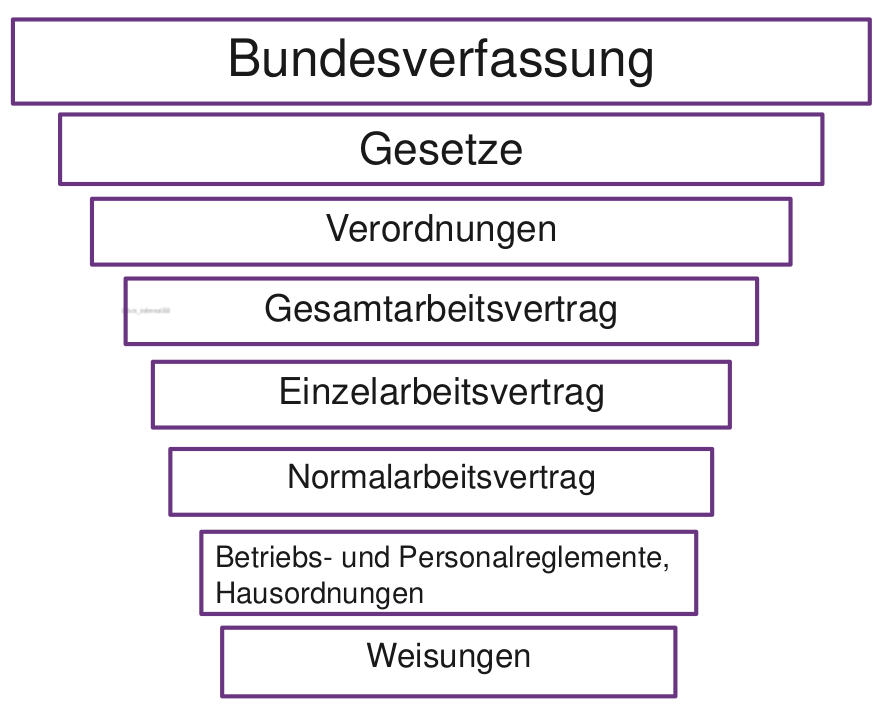
\includegraphics[width=10cm]{res/arbeitsrecht-vorrangigkeit.png}
  \caption{Vorrangigkeit der Rechtsgrundlagen}
\end{figure}

\subsection{Bundesgesetz über die Arbeit in Industrie, Gewerbe und Handel (Arbeitsgesetz ArG)}

\begin{description}
  \item[Verordnung 1] beinhaltet \textbf{Definition} und \textbf{Präzisierungen}, z.B. Begriffe Arbeitszeit, Pausen und Ruhezeiten, Nacht- und Sonntagsarbeit, Sonderschutz von Frauen, Aufgaben und Organisation der Behörden
  \item[Verordnung 2] sieht \textbf{Sonderbestimmungen} für einzelne Gruppen von Betrieben oder Arbeitnehmerinnen vor. Sie umschreibt die bei Vorliegen von besonderen Verhältnissen \textbf{möglichen Abweichungen von den gesetzlichen Arbeits- und Ruhezeitvorschriften} und bezeichnet die Betriebsarten oder Gruppen von Arbeitnehmern, welche unter diese Abweichungen fallen.
  \item[Verordnung 3] regelt die Rechte und Pflichten der Arbeitgeber und Arbeitnehmer zum \textbf{Gesundheitsschutz}, z.B. Anforderungen an Räume und Gebäude, Arbeitsplätze, Schutzausrüstung.
  \item[Verordnung 4] regelt auf industrielle Betriebe anwendbare Vorschriften sowie das Plangenehmigungsverfahren.
  \item[Verordnung 5] bezweckt den Schutz der \textbf{Gesundheit und der Sicherheit der Jugendlichen} bei der Arbeit bis zum 18. Altersjahr, z.B. gefährliche Arbeiten, Beschäftigung schulentlassener Jugendlicher unter 15 Jahren, Arbeits- und Ruhezeiten.
\end{description}

\subsection{Weitere Gesetze}
\begin{itemize} 
  \item Bundesgesetz betreffend die Ergänzung des Schweizerischen Zivilgesetzbuches, Fünfter Teil, Obligationenrecht
  \item Bundesgesetz über die Berufsbildung (BBG)
  \item Öffentlich-rechtliche Personalgesetze, z.B. Personalgesetz Kanton St. Gallen (PersG)
  \item Bundesgesetz über die Arbeitsvermittlung und den Personalverleih (Arbeitsvermittlungsgesetz, AVG)
  \item Bundesgesetz über den Datenschutz (Datenschutzgesetz DSG)
  \item Bundesgesetz über die Gleichstellung von Frau und Mann (Gleichstellungsgesetz, GlG)
  \item Verordnung des WBF über gefährliche und beschwerliche Arbeiten bei Schwangerschaft und Mitterschaft (Mutterschutzverordnung)
  \item Bundesgesetz über die Information und Mitsprache der Arbeitnehmerinnen und Arbeitnehmer in den Betrieben (Mitwirkungsgesetz, MWG)
\end{itemize}

\section{Entstehung eines Arbeitsverhältnisses}

\subsection{Einzelarbeitsvertrag EAV}
\textbf{OR 319 ff.}

Grundsätzlich formfrei, Sondervereinbarungen wie Verlängerung der Probezeit, Lohnverzicht bei
Überstunden oder Konkurrenzverbot, erfordern aber die schriftliche Form. 
Einigung betreffend der Hauptpunkte nötig, sonst kein Vertrag. Dies sind Parteien, Beginn und Dauer, Umfang, Arbeitsort, Lohn, Arbeitszeit und Ferien, Probezeit, Kündigungsfrist.
Weiter Anforderungen wie normale Verträge, OR 1-2.

\begin{description}
  \item[Besondere Einzelarbeitsverträge] sind Lehrvertrag (OR 344a Abs. 1), Handelsreisende (OR 347a Abs. 1), Heimarbeitsvertrag (OR 351a Abs. 1)
  \item[Gesamtarbeitsvertrag] Vertrag zwischen Arbeitgebern oder -verbänden und Arbeitnehmerverbänden zur Regelung der Arbeitsbedingugen. Einfache Schriftlichkeit. (OR 356c Abs. 1). Beispielregelungen: Anspruch 13. Monatslohn, Auszahlung Überstunden, Anzahl Ferienwochen, Haftung bei Schäden. 
  \item[Normalarbeitsvertrag] Behördlicher Erlass mit arbeitsvertraglichen Bestimmungen, diese können zwingenden oder empfehlenden Charakter haben. Zwei Arten: zwingende Mindestlöhne oder Bestimmungen über das Arbeitsverhältnis. Beispiel: NAV Hauswirtschaft, regelt Mindestlöhne für Hausangestellte in Privathaushalten.
\end{description}

\subsection{Pflichten des Arbeitnehmers}
\textbf{OR 321 - Persönliche Arbeitspflicht} 

\textit{Der Arbeitnehmer hat die vertraglich übernommene Arbeit in eigener Person zu leisten,
sofern nichts anderes verabredet ist oder sich aus den Umständen ergibt.}
\vspace{3mm}

\noindent
\textbf{OR 321d - Weisungen}

\textit{1 Der Arbeitgeber kann über die Ausführung der Arbeit und das Verhalten der Arbeitnehmer im Betrieb oder Haushalt allgemeine Anordnungen erlassen und ihnen besondere Weisungen erteilen. (Im Rahmen der betrieblichen Bedürfnisse)}

\noindent
Unzulässig sind bspw. Weisungen, welche die dem Arbeitnehmenden vertraglich eingeräumte
freie und selbstständige Stellung einschränken und in seinen vertraglich festgelegten
Kompetenzbereich eingreifen.

Das Weisungsrecht des Arbeitgebers wird durch das Persönlichkeitsrecht des Arbeitnehmenden
begrenzt. Dabei ist immer eine Interessenabwägung vorzunehmen.

Auch muss das Weisungsrecht nach Treu und Glauben ausgeübt werden. So sind willkürliche,
ohne sachliche Begründung erlassene oder gar schikanöse Weisungen unzulässig.
\vspace{3mm}

\noindent
\textbf{OR 321a - Sorgfalts- und Treuepflicht}

\textit{1 Der Arbeitnehmer hat die ihm übertragene Arbeit sorgfältig auszuführen und die berechtigten Interessen des Arbeitgebers in guten Treuen zu wahren.}

\textit{2 Er hat Maschinen, Arbeitsgeräte, technische Einrichtungen und Anlagen sowie Fahrzeuge des Arbeitgebers fachgerecht zu bedienen und diese sowie Material, die ihm zur Ausführung der Arbeit zur Verfügung gestellt werden, sorgfältig zu behandeln.}

\textit{3 Während der Dauer des Arbeitsverhältnisses darf der Arbeitnehmer keine Arbeit gegen Entgelt für einen Dritten leisten, soweit er dadurch seine Treuepflicht verletzt, insbesondere den Arbeitgeber konkurrenziert.}

\textit{4 Der Arbeitnehmer darf geheim zu haltende Tatsachen, wie namentlich Fabrikations- und Geschäfts- geheimnisse, von denen er im Dienst des Arbeitgebers Kenntnis erlangt, während des Arbeitsverhältnisses nicht verwerten oder anderen mitteilen; auch nach dessen Beendigung bleibt er zur Verschwiegenheit verpflichtet, soweit es zur Wahrung der berechtigten Interessen des Arbeitgebers erforderlich ist.}
\vspace{3mm}

\noindent
Unter Umständen auch für die Zeit nach Beendigung des Arbeitsverhältnisses, sog. abgeschwächte Geheimhaltungspflicht.

\noindent
Tatsachen gelten als geheim, wenn: 

diese weder offenkundig noch allgemein zugänglich sind und

an deren Geheimhaltung der Arbeitgeber (Geheimnisherr) ein berechtigtes Interesse hat und

diese geheim halten will.

Schliesslich muss das Geheimnis einen Bezug zum Unternehmen (Fabrikation oder Geschäft) aufweisen.

Solche Geheimnisse können etwa Kundenkarteien, Herstellungsverfahren, Algorithmen oder spezielles Know-how sein.
Das Bundesgericht fordert, dass diese Informationen einen Einfluss auf das Geschäftsergebnis haben können.
Die Gesetzesbestimmung zum Schutz von Geschäftsgeheimnissen ist offen formuliert, was zu Rechtsunsicherheiten führen kann. Um sicher zu gehen, sollten daher Geschäftsgeheimnisse explizit als solche gekennzeichnet werden und für jedermann identifizierbar sein.

\noindent
s. auch Art. 162 StGB Verletzung des Fabrikations- oder Geschäftsgeheimnis
\vspace{3mm}

\noindent
\textbf{OR 340 ff - Konkurrenzverbot}

\noindent
Vertragsklausel, die es dem Arbeitnehmer verbietet nach Beendigung des Arbeitsverhältnisses, für einen Dritten oder
selbstständig seine Arbeitgeberin zu konkurrenzieren.

\textit{1 Der handlungsfähige Arbeitnehmer kann sich gegenüber dem Arbeitgeber schriftlich verpflichten, nach Beendigung des Arbeitsverhältnisses sich jeder konkurrenzierenden Tätigkeit zu enthalten, insbesondere weder auf eigene Rechnung ein Geschäft zu betreiben, das mit dem des Arbeitgebers in Wettbewerb steht, noch in einem solchen Geschäft tätig zu sein oder sich daran zu beteiligen.}

\textit{2 Das Konkurrenzverbot ist nur verbindlich, wenn das Arbeitsverhältnis dem Arbeitnehmer Einblick in den Kundenkreis oder in Fabrikations- und Geschäftsgeheimnisse gewährt und die Verwendung dieser Kenntnisse den Arbeitgeber erheblich schädigen könnte.}
\vspace{3mm}

\noindent
Voraussetzung für ein gültiges Konkurrenzverbot:
\begin{itemize}
  \item Handlungsfähigkeit des Arbeitnehmers
  \item Schriftliche Vereinbarung (Unterschrift des Arbeitnehmers)
  \item Konkurrenzierende Tätigkeit (gleichartige Leistungen)
  \item Einblick in den Kundenkreis (Aussendienstmitarbeiter) oder in Fabrikations- und Geschäftsgeheimnisse (Kenntnisse über Rezepturen)
  \item Erhebliches Schädigungspotenzial für die Arbeitgeberin (die Kenntnisse selbst müssen dieses Potenzial haben)
  \item Angemessene Begrenzung nach Ort (Geschäftsbereich der Arbeitgeberin), Zeit (i.d.R. nicht mehr als drei Jahre) und Gegenstand (genaue Umschreibung)
\end{itemize}
\vspace{3mm}

\noindent
\textbf{OR 321e - Haftung des Arbeitnehmers aus Vertragsverletzung}

\textit{1 Der Arbeitnehmer ist für den Schaden verantwortlich, den er absichtlich oder fahrlässig dem Arbeitgeber zufügt.}

\textit{2 Das Mass der Sorgfalt, für die der Arbeitnehmer einzustehen hat, bestimmt sich nach dem einzelnen Arbeitsverhältnis, unter Berücksichtigung des Berufsrisikos, des Bildungsgrades oder der Fachkenntnisse, die zu der Arbeit verlangt werden, sowie der Fähigkeiten und Eigenschaften des Arbeitnehmers, die der Arbeitgeber gekannt hat oder hätte kennen sollen.}

Gewisse Kriterien gelten, um die Haftung zu bestimmen:

\begin{itemize}
  \item Berücksichtigung des konkreten Arbeitsverhältnisses
  \item Berufsrisiko
  \item Bildungsgrad oder Fachkenntnisse
  \item Lohnhöhe
  \item Mitverschulden des Arbeitgebers
  \item Einwilligung oder Anordnung des Arbeitgebers
  \item Kenntnisse des Arbeitgebers über die Fähigkeiten und Eigenschaften des Arbeitnehmers
\end{itemize}

Faustregeln Fahrlässigkeit:
\begin{description}
  \item[Absicht:] Schaden ist mit voller Absicht geschehen oder in Kauf genommen worden. Schadenersatz in voller Höhe fällig.
  \item[Grobe Fahrlässigkeit:] Das darf einfach nicht passieren, "wie kann man nur". Schadenersatz grundsätzlich in voller Höhe, meist aber maximal 3 Monatslöhne.
  \item[Mittlere Fahrlässigkeit:] So etwas sollte eigentlich nicht passieren. Schadenersatz Hälfe bis 2/3 des Schadens, maximal 2 Monatslöhne.
  \item[Leichte Fahrlässigkeit:] Das kann mal passieren, man hätte besser aufpassen können. Schadenersatz bis zur Hälfte der Summe, maximal 1 Monatslohn.
  \item[Bagatellfälle:] Das bringt die Arbeit schon einmal mit sich. Kein Schadenersatz geschuldet.     
\end{description}

Forderungen für absichtlich zugefügte Schäden dürfen ohne Einschränkung mit den Lohnforderungen des Arbeitnehmers verrechnet werden. Für fahrlässige Schadenverursachung bildet der pfändbare Lohn (Existenzminimum) die Grenze.
\vspace{3mm}

\textbf{OR 321c - Überstundenarbeit}

\textit{1 Wird gegenüber dem zeitlichen Umfang der Arbeit, der verabredet oder üblich oder durch Normalarbeitsvertrag oder Gesamtarbeitsvertrag bestimmt ist, die Leistung von Überstundenarbeit notwendig, so ist der Arbeitnehmer dazu soweit verpflichtet, als er sie zu leisten vermag und sie ihm nach Treu und Glauben zugemutet werden kann.}

\textit{2 Im Einverständnis mit dem Arbeitnehmer kann der Arbeitgeber die Überstundenarbeit innert eines angemessenen Zeitraumes durch Freizeit von mindestens gleicher Dauer ausgleichen.}

\textit{3 Wird die Überstundenarbeit nicht durch Freizeit ausgeglichen und ist nichts anderes schriftlich verabredet oder durch Normalarbeitsvertrag oder Gesamtarbeitsvertrag bestimmt, so hat der Arbeitgeber für die Überstundenarbeit Lohn zu entrichten, der sich nach dem Normallohn samt einem Zuschlag von mindestens einem Viertel bemisst.}

\begin{description}
  \item[Überstunden (OR)] sind zu leisten wenn erforderlich, zumutbar, machbar (keine Überforderung), und die Bestimmungen des ArG eingehalten werden (Arbeits- und Ruhezeiten). Abgeltung kann vertraglich festgelegt werden. Wenn nichts anderes vereinbart gilt Auszahlung mit 25\% Zuschlag.
  \item[Überzeit (ArG)] beschreibt Zeit, die die gesetzliche Höchstarbeitszeit überschreitet. Entschädigung kann nicht vertraglich wegbedungen werden. Teilwese aber: nur Entschädigt, wenn mehr als 60 Stunden im Jahr. Zwingende Bestimmungen im ArG: Dringlichkeit wie Inventaraufnahmen, Rechnungsabschlüsse, Vermeidung oder Beseitigung von Betriebsstörungen. Darf nicht mehr als 2 Stunden pro Tag oder 170 Stunden im Jahr betragen wenn 45h wöchentliche Höchstarbeitszeit gelten, 140 Stunden im Jahr bei 50h wöchentlicher Höchstarbeitszeit. 
\end{description}

\subsection{Pflichten des Arbeitgebers}

\noindent
\textbf{OR 322 ff - Lohn}

Lohnarten sind Stunden-, Fix- oder Akkordlohn, Anteil am Geschäftsergebnis, Individuelle Erfolgsbeteiligung, Provision \textit{(OR 322b)}, Gratifikation \textit{(OR 322d)}, Naturallohn (Kost und Logis), Lohnzulagen (Überstundenentschädigung, Nacht- und Sonntagsarbeitszuschläge, Schichtzulagen, Feiertags- und Ferienvergütungen), Fringe Benefits (Vergünstigungen, Repräsentationsspesen, Clubmitgliedschaften etc.) 

\textit{322 - 1 Der Arbeitgeber hat dem Arbeitnehmer den Lohn zu entrichten, der verabredet oder üblich oder durch Normalarbeitsvertrag oder Gesamtarbeitsvertrag bestimmt ist.}

\textit{323 - 1 Sind nicht kürzere Fristen oder andere Termine verabredet oder üblich und ist durch Normalarbeitsvertrag oder Gesamtarbeitsvertrag nichts anderes bestimmt, so ist dem Arbeitnehmer der Lohn Ende jedes Monats auszurichten.}

\textit{2 Ist nicht eine kürzere Frist verabredet oder üblich, so ist die Provision Ende jedes Monats auszurichten; erfordert jedoch die Durchführung von Geschäften mehr als ein halbes Jahr, so kann durch schriftliche Abrede die Fälligkeit der Provision für diese Geschäfte hinausgeschoben werden.}

\textit{3 Der Anteil am Geschäftsergebnis ist auszurichten, sobald dieses festgestellt ist, spätestens jedoch sechs Monate nach Ablauf des Geschäftsjahres.}

\textit{4 Der Arbeitgeber hat dem Arbeitnehmer nach Massgabe der geleisteten Arbeit den Vorschuss zu gewähren, dessen der Arbeitnehmer infolge einer Notlage bedarf und den der Arbeitgeber billigerweise zu gewähren vermag.}

\begin{description}
  \item[Lohn bei Verhinderung der Annahme der Arbeitsleistung:] dazu gilt OR 324. Lohn ist geschuldet, keine Nachholpflicht des Arbeitnehmers. Kein Gläubigerverzug jedoch bei Krieg, Einfuhrverboten, oder wenn die Annahme der Leistung mit unzumutbaren rechtlichen Risiken verbunden ist. 
  \item[Lohn bei Verhinderung des Arbeitnehmers] Bei Gründen die in seiner Person liegen besteht grundsätzlich eine Lohnfortzahlungspflicht. Gründe sind Krankheit, ärztlich verordneter Erholungsurlaub, Unfall, Schwangerschaftsabsenz (ärztl. Attestiert), Arztbesuch, Umzug, Heirat, temporäre Pflege eines erkrankten Angehörigen etc.
  Kein Verschulden: Verkehrsunfälle, "normale" Sportunfälle. Verschulden: Risikosport, Fahren in angetrunkenem Zustand, Skitouren bei grosser Lawinengefahr \ldots 
  
  \item[Lohnfortzahlung] im ersten Dienstjahr drei Wochen (OR 324a Abs. 2)
  Danach gemäss Skala, alternativ mindestens eine vertraglich gleichwertige Lösung.
  \begin{itemize}
    \item Taggelder mindestens im Umfang von 80\% des Lohnes
    \item während mindestens 720 Tagen innert 900 Tagen
    \item bei mindestens hälftiger Prämienteilung
    \item max. 3 Karenztage
  \end{itemize}
  
  \noindent
  Lohnfortzahlungspflicht entsteht in jedem Dienstjahr von neuem. Anspruch besteht nicht pro Ereignis, sondern gesamthaft. Der Anspruch besteht bei teilweiser Verhinderung nicht für eine bestimmte Zeit, sondern verlängert sich bis der Anspruch auf die volle Lohnzahlung abgegolten ist.
\end{description}
  
\begin{figure}
  \centering
  \includegraphics*[width=12cm]{res/arbeitsrecht-lohnfortzahlung-skalen.png}
  \caption{Verschiedene Skalen zur Lohnfortzahlung}
\end{figure}

\noindent
\textbf{OR 328 - Schutz der Persönlichkeit des Arbeitnehmers}

\textit{1 Der Arbeitgeber hat im Arbeitsverhältnis die Persönlichkeit des Arbeitnehmers zu achten und zu schützen, auf dessen Gesundheit gebührend Rücksicht zu nehmen und für die Wahrung der Sittlichkeit zu sorgen. Er muss insbesondere dafür sorgen, dass Arbeitnehmerinnen und Arbeitnehmer nicht sexuell belästigt werden und dass den Opfern von sexuellen Belästigungen keine weiteren Nachteile entstehen.}

\textit{2 Er hat zum Schutz von Leben, Gesundheit und persönlicher Integrität der Arbeitnehmerinnen und Arbeitnehmer die Massnahmen zu treffen, die nach der Erfahrung notwendig, nach dem Stand der Technik anwendbar und den Verhältnissen des Betriebes oder Haushaltes angemessen sind, soweit es mit Rücksicht auf das einzelne Arbeitsverhältnis und die Natur der Arbeitsleistung121 ihm billigerweise zugemutet werden kann.}
\vspace{3mm}

\newpage
\noindent
\textbf{OR 330a - Erstellen eines Arbeitszeugnisses}

\textit{Der Arbeitnehmer kann jederzeit vom Arbeitgeber ein Zeugnis verlangen, das sich über die Art und Dauer des
Arbeitsverhältnisses sowie über seine Leistungen und sein Verhalten ausspricht.}

\textit{2 Auf besonderes Verlangen des Arbeitnehmers hat sich das Zeugnis auf Angaben über die Art und Dauer des Arbeitsverhältnisses zu beschränken.}
\vspace{3mm}

Ein Vollzeugnis sollte folgende Angaben enthalten: Identität des Arbeitnehmers und Arbeitgebers, Beginn und Ende des Arbeitsverhältnisses, detaillierte Auflistung der wichtigsten Funktionen, der das Arbeitsverhältnis prägenden Tätigkeiten und deren Zeitdauer, eine aussagekräftige Bewertung der Leistung und des Verhaltens, die rechtsgültige Unterschrift des Arbeitgebers.

\begin{figure}[H]
  \centering
  \includegraphics*[width=\linewidth]{res/arbeitsrecht-arbeitszeugnis.png}
  \caption{Anforderungen an ein Arbeitszeugnis}
\end{figure}

\newpage
\subsection{Spezielle Bestimmungen}

\textbf{OR 361} in jedem Fall unabänderlich:
Durch Abrede, Normalarbeitsvertrag oder Gesamtarbeitsvertrag darf von den folgenden Vorschriften weder zuungunsten des Arbeitgebers noch des Arbeitnehmers abgewichen werden:
\begin{description}
    \item[Artikel 321c]
    Absatz 1 (Überstundenarbeit)

    \item[Artikel 323]
    Absatz 4 (Vorschuss)

    \item[Artikel 323b]
    Absatz 2 (Verrechnung mit Gegenforderungen)

    \item[Artikel 325]
    Absatz 2 (Abtretung und Verpfändung von Lohnforderungen)

    \item[Artikel 326]
    Absatz 2 (Zuweisung von Arbeit)

    \item[Artikel 329d]
    Absätze 2 und 3 (Ferienlohn)

    \item[Artikel 331]
    Absätze 1 und 2 (Zuwendungen für die Personalfürsorge)

    \item[Artikel 331b]
    (Abtretung und Verpfändung von Forderungen auf Vorsorgeleistungen)

    \item[Artikel 334]
    Absatz 3 (Kündigung beim langjährigen Arbeitsverhältnis)

    \item[Artikel 335]
    (Kündigung des Arbeitsverhältnisses)

    \item[Artikel 335k]
    (Sozialplan während eines Konkurs- oder eines Nachlassverfahrens)

    \item[Artikel 336]
    Absatz 1 (Missbräuchliche Kündigung)

    \item[Artikel 336a]
    (Entschädigung bei missbräuchlicher Kündigung)

    \item[Artikel 336b]
    (Geltendmachung der Entschädigung)

    \item[Artikel 336d]
    (Kündigung zur Unzeit durch den Arbeitnehmer)

    \item[Artikel 337]
    Absätze 1 und 2 (Fristlose Auflösung aus wichtigen Gründen)

    \item[Artikel 337b]
    Absatz 1 (Folgen bei gerechtfertigter Auflösung)

    \item[Artikel 337d]
    (Folgen bei ungerechtfertigtem Nichtantritt oder Verlassen der Arbeitsstelle)

    \item[Artikel 339]
    Absatz 1 (Fälligkeit der Forderungen)

    \item[Artikel 339a]
    (Rückgabepflichten)

    \item[Artikel 340b]
    Absätze 1 und 2 (Folgen der Übertretung des Konkurrenzverbotes)

    \item[Artikel 342]
    Absatz 2 (Zivilrechtliche Wirkungen des öffentlichen Rechts)

    \item[Artikel 346]
    (Vorzeitige Auflösung des Lehrvertrages)

    \item[Artikel 349c]
    Absatz 3 (Verhinderung an der Reisetätigkeit)

    \item[Artikel 350]
    (Besondere Kündigung)

    \item[Artikel 350a]
    Absatz 2 (Rückgabepflichten)
\end{description}

\textit{2 Abreden sowie Bestimmungen von Normalarbeitsverträgen und Gesamtarbeitsverträgen, die von den vorstehend angeführten Vorschriften zuungunsten des Arbeitgebers oder des Arbeitnehmers abweichen, sind nichtig.}

\newpage
\textbf{OR 362} abänderlich zu Gunsten des Arbeitnehmers: Durch Abrede, Normalarbeitsvertrag oder Gesamtarbeitsvertrag darf von den folgenden Vorschriften nicht zuungunsten der Arbeitnehmerin oder des Arbeitnehmers abgewichen werden:
\begin{description}
  \item[Artikel 321e]
    (Haftung des Arbeitnehmers)

    \item[Artikel 322a]
    Absätze 2 und 3 (Anteil am Geschäftsergebnis)

    \item[Artikel 322b]
    Absätze 1 und 2 (Entstehung des Provisionsanspruchs)

    \item[Artikel 322c]
    (Provisionsabrechnung)

    \item[Artikel 323b]
    Absatz 1 zweiter Satz (Lohnabrechnung)

    \item[Artikel 324]
    (Lohn bei Annahmeverzug des Arbeitgebers)

    \item[Artikel 324a]
    Absätze 1 und 3 (Lohn bei Verhinderung des Arbeitnehmers)

    \item[Artikel 324b]
    (Lohn bei obligatorischer Versicherung des Arbeitnehmers)

    \item[Artikel 326]
    Absätze 1, 3 und 4 (Akkordlohnarbeit)

    \item[Artikel 326a]
    (Akkordlohn)

    \item[Artikel 327a]
    Absatz 1 (Auslagenersatz im Allgemeinen)

    \item[Artikel 327b]
    Absatz 1 (Auslagenersatz bei Motorfahrzeug)

    \item[Artikel 327c]
    Absatz 2 (Vorschuss für Auslagen)

    \item[Artikel 328]
    (Schutz der Persönlichkeit des Arbeitnehmers im Allgemeinen)

    \item[Artikel 328a]
    (Schutz der Persönlichkeit bei Hausgemeinschaft)

    \item[Artikel 328b]
    (Schutz der Persönlichkeit bei der Bearbeitung von Personendaten)

    \item[Artikel 329]
    Absätze 1, 2 und 3 (Freizeit)

    \item[Artikel 329a]
    Absätze 1 und 3 (Dauer der Ferien)

    \item[Artikel 329b]
    Absätze 2 und 3 (Kürzung der Ferien)

    \item[Artikel 329c]
    (Zusammenhang und Zeitpunkt der Ferien)

    \item[Artikel 329d]
    Absatz 1 (Ferienlohn)

    \item[Artikel 329e]
    Absätze 1 und 3 (Jugendurlaub)

    \item[Artikel 329f]
    (Mutterschaftsurlaub)

    \item[Artikel 329g]
    (Vaterschaftsurlaub)

    \item[Artikel 329h]
    (Urlaub für die Betreuung von Angehörigen)

    \item[Artikel 329i]
    (Urlaub für die Betreuung eines wegen Krankheit oder Unfall gesundheitlich schwer beeinträchtigten Kindes)

    \item[Artikel 329j]
    (Adoptionsurlaub)

    \item[Artikel 330]
    Absätze 1, 3 und 4 (Kaution)

    \item[Artikel 330a]
    (Zeugnis)

    \item[Artikel 331]
    Absätze 3 und 4 (Beitragsleistung und Auskunftspflicht bei Personalfürsorge)

    \item[Artikel 331a]
    (Beginn und Ende des Vorsorgeschutzes)

    \item[Artikel 332]
    Absatz 4 (Vergütung bei Erfindungen)

    \item[Artikel 333]
    Absatz 3 (Haftung bei Übergang des Arbeitsverhältnisses)

    \item[Artikel 335c]
    Absatz 3 (Kündigungsfristen)

    \item[Artikel 335i]
    (Verhandlungspflicht zwecks Abschlusses eines Sozialplans)

    \item[Artikel 335j]
    (Aufstellung des Sozialplans durch ein Schiedsgericht)

    \item[Artikel 336]
    Absatz 2 (Missbräuchliche Kündigung durch den Arbeitgeber)

    \item[Artikel 336c]
    (Kündigung zur Unzeit durch den Arbeitgeber)

    \item[Artikel 337a]
    (Fristlose Auflösung wegen Lohngefährdung)

    \item[Artikel 337c]
    Absatz 1 (Folgen bei ungerechtfertigter Entlassung)

    \item[Artikel 338]
    (Tod des Arbeitnehmers)

    \item[Artikel 338a]
    (Tod des Arbeitgebers)

    \item[Artikel 339b]
    (Voraussetzungen der Abgangsentschädigung)

    \item[Artikel 339d]
    (Ersatzleistungen)

    \item[Artikel 340]
    Absatz 1 (Voraussetzungen des Konkurrenzverbotes)

    \item[Artikel 340a]
    Absatz 1 (Beschränkung des Konkurrenzverbotes)

    \item[Artikel 340c]
    (Wegfall des Konkurrenzverbotes)

    \item[Artikel 341]
    Absatz 1 (Unverzichtbarkeit)

    \item[Artikel 345a]
    (Pflichten des Lehrmeisters)

    \item[Artikel 346a]
    (Lehrzeugnis)

    \item[Artikel 349a]
    Absatz 1 (Lohn des Handelsreisenden)

    \item[Artikel 349b]
    Absatz 3 (Ausrichtung der Provision)

    \item[Artikel 349c]
    Absatz 1 (Lohn bei Verhinderung an der Reisetätigkeit)

    \item[Artikel 349e]
    Absatz 1 (Retentionsrecht des Handelsreisenden)

    \item[Artikel 350a]
    Absatz 1 (Provision bei Beendigung des Arbeitsverhältnisses)

    \item[Artikel 352a]
    Absatz 3 (Haftung des Heimarbeitnehmers)

    \item[Artikel 353]
    (Abnahme des Arbeitserzeugnisses)

    \item[Artikel 353a]
    (Ausrichtung des Lohnes)

    \item[Artikel 353b]
    Absatz 1 (Lohn bei Verhinderung an der Arbeitsleistung)
\end{description}

\textit{2 Abreden sowie Bestimmungen von Normalarbeitsverträgen und Gesamtarbeitsverträgen, die von den vorstehend angeführten Vorschriften zuungunsten des Arbeitnehmers abweichen, sind nichtig.}


\section{Beendigung des Arbeitsverhältnis}
\subsection{Die Kündigung}
Grundsätzlich gilt in der Schweiz bei privatrechtlichen Arbeitsverhältnissen das Prinzip der Kündigungsfreiheit. Es wird zur Auflösung kein \textit{besonderer} Grund benötigt, der darf aber nicht \textit{missbräuchlich} sein.

Eine Kündigung ist eine \textbf{einseitige empfangsbedürftige Willenskundgabe}.

Gilt für die Beendigung des Arbeitsverhältnisses ein Endtermin, wie das Ende eines Monats, muss die Kündigung am letzten Tag dieses Monats der Gegenseite \textit{zur Kenntnis gebracht} werden, nicht erst versendet worden sein.

Wenn nichts anderes vereinbart ist die Kündigung Formfrei möglich, eine schriftliche Begründung kann verlangt werden \textit{(OR 335 Abs. 2)}.

\begin{description}
  \item[Während der Probezeit (OR 335b)], wenn nicht anders bestimmt gilt dabei der erste Monat eines unbefristeten Arbeitsverhältnisses. Maximal 3 Monate. Verlängerung nur durch unter OR 335b Abs. 3 beschriebene Gründe.
  
  \textit{Kündigungsfrist}: 7 Kalendertage. Kann durch schriftliche Abrede, NAV oder GAV gekürzt, verlängert oder wegbedungen werden. Kein Kündigungsschutz für den Arbeitnehmer.
  
  \item[Nach der Probezeit] gelten verschiedene Kündigungsfristen: 1 Monat im 1. Dienstjahr, 2 Monate im 2. bis 9. Dienstjahr, 3 Monate ab dem 10. Dienstjahr. Durch schriftliche Abrede können die Fristen verändert werden, jedoch nicht unter einen Monat (ausser wenn durch GAV vereinbart und nur im ersten Dienstjahr.) 
  
  \item[Missbräuchliche Kündigung]
  Beispiele: nach 44 Dienstjahren kurz vor der Pension, ohne zureichenden Grund. Rachekündigung, wenn der Arbeitnehmer von geltendem Recht gebrauch macht. Vereitelungskündigung, um einen entstehenden Anspruch der anderen Partei zu verhindern. Das Ausüben eines verfassungsmässigen Rechtes der anderen Partei ist ebenfalls kein gültiger Kündigungsgrund. Einem Arbeitnehmer ist es also grundsätzlich erlaubt, Kritik am Arbeitgeber im Rahmen seiner Meinungsäusserungsfreiheit auszuüben. Dieser darf jedoch dabei seine Treuepflicht nicht verletzen. 
  \begin{figure}[H]
    \centering
    
\includegraphics[width=12cm]{res/arbeitsrecht-missbr-kuendigung-fristen.png}
    \caption{Fristen bei Missbräuchlicher Kündigung}
  \end{figure}

  Wer die Missbräuchlichkeit einer Kündigung geltend machen will, muss zwei Fristen zwingend einhalten. Die Einsprachefrist dauert bis zum Ablauf der Kündigungsfrist, die Klagefrist endet 180 Tage nach Beendigung des Arbeitsverhältnisses.

  Rechtsfolgen: Selbst wenn das Gericht eine Kündigung als missbräuchlich qualifiziert, ist diese rechtswirksam. Der Arbeitnehmer hat Anspruch auf Entschädigungszahlung, maximal sechs Monatslöhne. Festlegung liegt im Ermessen des Richters, der die Umstände zu berücksichtigen hat. 

  \item[Kündigung zur Unzeit] Bei Arbeitsverhinderungen infolge Krankheit und
Unfall, bei Schwangerschaft und Mutterschaft sowie bei Dienstleistungen für Hilfsaktionen
im Ausland besteht ein zeitlich begrenzter Kündigungsschutz \textit{(OR 336c)}. Dieser gilt genauso für Teilzeit- und Temporärarbeitsverträgen sowie bei Freistellung.
\textbf{Keine Anwendung} hat der Kündigungsschutz bei befristeten Arbeitsverhältnissen, Aufhebungsverträgen und bei gerechtfertigten fristlosen Entlassungen.
\textbf{Gilt} erst nach Ablauf der Probezeit und nur bei einer Arbeitgeberkündigung \textit{(OR 336c Abs. 1)}.

Sperrfristen: 
\begin{itemize}
  \item 4 Wochen vor, während und 4 Wochen nach Militär, Zivilschutz oder Zivildienst. 
  \item Bei Krankheit oder Unfall 30 Tage im 1. Dienstjahr, 90 Tage vom 2. bis und mit 5. Dienstjahr, 180 Tage ab dem 6. Dienstjahr
  \item Bei Schwangerschaft und Niederkunft während der ganzen Dauer der Schwangerschaft und bis 16 Wochen nach der Geburt
  \item Bei Dienstleistungen für Hilfsaktionen im Ausland für die Dauer der Dienstleistung
\end{itemize}
Weitere Facts: 
\begin{itemize}
  \item Ist ein Arbeitnehmer zum Zeitpunkt der Kündigung krank, ist die Kündigung, sofern nach Ablauf der Probezeit und durch den Arbeitgeber ausgesprochen, nichtig. (Art. 336c Abs. 2 OR)
  \item Ist die Kündigung gültig erfolgt und der Arbeitnehmer wird noch vor dem Beginn der Kündigungsfrist (a) krank, hat das keine Verlängerung der Kündigungsfrist zur Folge.
  \item Ist der Arbeitnehmer in der Kündigungsfrist krank, wird die Dauer der Krankheit zum eigentlichen Ende des Arbeitsverhältnisses (b) hintangestellt und verlängert dasselbe grds. um diese Dauer. Ist das Arbeitsverhältnis per Ende Monat kündbar, gilt er auf b folgende Monat als neues Ende.
\end{itemize}
\item[Ausserordentliche, fristlose Kündigung] OR 337

  \textit{1 Aus wichtigen Gründen kann der Arbeitgeber wie der Arbeitnehmer jederzeit das Arbeitsverhältnis fristlos auflösen; er muss die fristlose Vertragsauflösung schriftlich begründen, wenn die andere Partei dies verlangt.}

  \textit{2 Als wichtiger Grund gilt namentlich jeder Umstand, bei dessen Vorhandensein dem Kündigenden nach Treu und Glauben die Fortsetzung des Arbeitsverhältnisses nicht mehr zugemutet werden darf.}

  \textit{3 Über das Vorhandensein solcher Umstände entscheidet der Richter nach seinem Ermessen, darf aber in keinem Fall die unverschuldete Verhinderung des Arbeitnehmers an der Arbeitsleistung als wichtigen Grund anerkennen.}

  Beispiele für wichtige Gründe \textbf{auf Arbeitgeberseite}: Veruntreuung am Arbeitsplatz, Annahme von Schmiergeldern, Unwahre Angaben bei der Anstellung, Eigenmächtiger Ferienbezug, Verrat von Geschäftsgeheimnissen, Grobe Missachtung einer Weisung, Weniger schwerwiegende Verfehlungen aber nach erfolgter Abmahnung (heikel): Übermässiges privates Telefonieren, ungepflegtes Erscheinen wo relevant, grössere Verspätungen, verstoss gegen Weisungen (beharrliche oder wiederholte Nichtbeachtung von berechtigten Weisungen)

  Beispiele für wichtige Gründe \textbf{auf Arbeitnehmerseite}: Beschimpfungen und Tätlichkeiten durch den Arbeitgeber, unsittliche Anträge oder Belästigungen durch den Arbeitgeber, Kränkung und Belästigung durch Mitarbeiter ohne Eingreifen des Arbeitgebers, Weisungen, sittenwidrige oder strafbare Handlungen zu begehen, nicht behobene Sicherheitsmängel, unzumutbares Arbeitsklima ohne Eingreifen des AG, zu weitgehende Überwachung, schwerwiegende grundlose Verdächtigung oder üble Nachrede ... 
  
  Bei geringeren Problemen hat auch der Arbeitnehmer zuerst eine Verwarnung auszusprechen.

  \textbf{Folgen:} Wenn gerechtfertigt: \textit{(OR 337b)} \textit{1 Liegt der wichtige Grund zur fristlosen Auflösung des Arbeitsverhältnisses im vertragswidrigen Verhalten einer Vertragspartei, so hat diese vollen Schadenersatz zu leisten, unter Berücksichtigung aller aus dem Arbeitsverhältnis entstehenden Forderungen.}

  Wenn ungerechtfertigt: \textit{(OR 337c)} \textit{1 Entlässt der Arbeitgeber den Arbeitnehmer fristlos ohne wichtigen Grund, so hat dieser Anspruch auf Ersatz dessen, was er verdient hätte, wenn das Arbeitsverhältnis unter Einhaltung der Kündigungsfrist oder durch Ablauf der bestimmten Vertragszeit beendigt worden wäre.}

  \textit{2 Der Arbeitnehmer muss sich daran anrechnen lassen, was er infolge der Beendigung des Arbeitsverhältnisses erspart hat und was er durch anderweitige Arbeit verdient oder zu verdienen absichtlich unterlassen hat.}

  \textit{3 Der Richter kann den Arbeitgeber verpflichten, dem Arbeitnehmer eine Entschädigung zu bezahlen, die er nach freiem Ermessen unter Würdigung aller Umstände festlegt; diese Entschädigung darf jedoch den Lohn des Arbeitnehmers für sechs Monate nicht übersteigen.}

\end{description}

\section{Rechte an Erfindungen und Designs}

Erfindungen und Designs müssen einen Teil selbständig, kreativ und schöpferisch tätig sein. \textbf{Erfindung} bedeutet das Erzielen von wesentlichem technischen Fortschritt. \textbf{Design} ist Gestaltung von Erzeugnissen oder Teilen davon.

\vspace{3mm}
\textbf{OR 332}

\textit{1 Erfindungen und Designs, die der Arbeitnehmer bei \textbf{Ausübung seiner dienstlichen Tätigkeit und in Erfüllung seiner vertraglichen Pflichten} macht oder an deren Hervorbringung er mitwirkt, gehören unabhängig von ihrer Schutzfähigkeit dem Arbeitgeber.}

\textit{2 Durch \textbf{schriftliche Abrede} kann sich der Arbeitgeber den Erwerb von Erfindungen und Designs ausbedingen, die vom Arbeitnehmer bei Ausübung seiner dienstlichen Tätigkeit, aber nicht in Erfüllung seiner vertraglichen Pflichten gemacht werden.}

\textit{3 Der Arbeitnehmer, der eine Erfindung oder ein Design gemäss Absatz 2 macht, hat davon dem Arbeitgeber \textbf{schriftlich Kenntnis} zu geben; dieser hat ihm innert sechs Monaten schriftlich mitzuteilen, ob er die Erfindung beziehungsweise das Design erwerben will oder sie dem Arbeitnehmer freigibt.}

\textit{4 Wird die Erfindung oder das Design dem Arbeitnehmer nicht freigegeben, so hat ihm der Arbeitgeber eine besondere \textbf{angemessene Vergütung} auszurichten; bei deren Festsetzung sind alle Umstände zu berücksichtigen, wie namentlich der wirtschaftliche Wert der Erfindung beziehungsweise des Designs, die Mitwirkung des Arbeitgebers, die Inanspruchnahme seiner Hilfspersonen und Betriebseinrichtungen, sowie die Aufwendungen des Arbeitnehmers und seine Stellung im Betrieb.}

\begin{description}
  \item[Dienst- oder Aufgabenerfidungen] Das sind Erfindungen oder Designs, welche erstens in Ausübung der dienstlichen Tätigkeit und zweitens in Erfüllung der arbeitsvertraglichen Pflichten entstanden sind. Das Gesetz sieht bei der Aufgabenerfindung oder dem Aufgabendesign keinen Anspruch auf eine besondere Vergütung vor. Den Parteien steht es jedoch frei, eine abweichende Vereinbarung zu treffen.
  
  Erfindet ein Ingenieur während seiner Arbeitszeit eine Verbesserung einer bestehenden Maschine oder eine ganz neue Maschine, oder programmiert ein Softwareentwickler während seiner Arbeitszeit einen neuen Algorithmus, oder kreiert ein Werber während seiner Arbeitszeit eine bahnbrechende neue Kampagne, so sind das allesamt Diensterfindungen.

  \item[Gelgenheitserfindungen] Die Gelegenheitserfindung (entsteht eher zufällig) entsteht zwar auch während der Arbeitszeit (in Ausübung der dienstlichen Tätigkeit), gehört aber eben nicht zum Aufgabengebiet eines Arbeitnehmenden und entstand somit nicht in Erfüllung der arbeitsvertraglichen Pflichten. Sie stehen dem Arbeitnehmer als Erfinder zu. 
  Durch schriftliche Abrede kann sich der Arbeitgeber den Erwerb dieser Erfindung bzw. dieses Designs vorbehalten.

  In Bezug auf die Beispiele für die Diensterfindungen ist eine Gelegenheitserfindung die neue Maschine, erfunden durch einen Servicetechniker (der ist nicht für das Engineering neuer Maschinen zuständig ist), der Algorithmus eines Supporters (der nicht für die Software-Entwicklung zuständig ist) oder die Werbekampagne eines Buchhalters (der keine kreative Werbung machen muss).
  
  \item[Freie (arbeitsfremde) Erfindungen] Erfindungen oder Designs ohne sachlichen oder inhaltlichen Zusammenhang mit dem Arbeitsverhältnis stehen dem Arbeitnehmer zu. Durch Vereinbarung kann sich der Arbeitgeber auch die Rechte an freien Erfindungen und Designs übertragen lassen.
\end{description}